% !TeX root = ../main.tex

\xchapter{绪论}{Introduction}

视觉和语言是人类感知和理解环境的两种主要模态。为了使人工智能系统像人一样理解和利用视觉和语言信息,研究者们已经在计算机视觉和自然语言处理领域展开了大量的研究并取得了一系列先进成果。
这些成果为计算机视觉和自然语言处理交叉的视觉语言领域的发展奠定了坚实的基础。
本文聚焦视觉语言领域极具代表性的视觉问答任务,基于图网络和视觉语言预训练模型深入探讨了该任务面临的挑战:对视频中多粒度视觉语言信息的利用不充分、语言偏见导致的泛化能力不足、对视觉语言输入变化的鲁棒性不足以及少样本迁移学习能力不足,并提出了对应的解决方案。

% 本文面向视觉语言领域一个极具代表性的任务,即视觉问答(Visual Question Answering,VQA)任务,基于图网络和视觉语言预训练模型深入探讨了视觉问答面临的四大挑战:对视频中多粒度视觉语言信息的利用不充分、语言偏见导致的泛化能力不足、对视觉语言输入变化的鲁棒性不足以及少样本迁移学习能力不足,并提出了对应的解决方案。


% ******************************************************************
\xsection{研究背景及意义}{Background and Significance}

计算机视觉(Computer Vision,CV)和自然语言处理(Natural Language Processing, NLP)是人工智能的两大重要分支~\cite{li2022vision}。
在过去十几年中,人工智能和深度学习技术的发展和完善极大地推进了计算机视觉和自然语言处理领域中许多基础任务的研究进程,并取得了一系列先进的成果。
2015年,ResNet 模型~\cite{he2016deep}在ImageNet 数据集~\cite{deng2009imagenet}上以3.57\% 的错误率在计算机视觉领域的图像识别任务上达到人类水平。
2018年,微软团队在WMT-17的新闻数据集上以69.9\%的准确率在自然语言处理领域的机器翻译任务上达到人类水平~\cite{hassan2018achieving}。
基础任务的突破和计算机单模态学习能力的增强激发了研究者对计算机视觉和自然语言处理交叉领域(即,视觉语言领域,Vision and Language)的探索和研究。
同时,随着大数据和互联网的快速发展,视频、图像、文本、语音等多种形式的多媒体数据呈爆炸式增长。
从应用的角度出发,对海量的多模态数据进行有效感知、理解和利用也成为了人工智能研究的一个重点。因此,视觉语言领域的许多任务得到越来越多的关注,如跨模态检索~\cite{frome2013devise}、图像描述~\cite{vinyals2016show}、视觉问答~\cite{antol2015vqa}、视觉语言导航~\cite{anderson2018vision}等。
其中,视觉问答(Visual Question Answering,VQA)作为视觉语言领域的代表性任务之一,因涉及多模态理解和推理且性能易于评估等原因成为了近几年的研究热点。
% 基于计算机视觉(CV)和自然语言处理(NLP)的视觉问答(Visual Question Answering, VQA)是人工智能研究领域的新兴课题。跨模态


视觉问答的概念最早于2014年由Mateusz和Mario~\cite{malinowski2014multi}提出。如图~\ref{fig:c1_vqa}中的示例所示,视觉问答的目标是,给定一个视频片段(图~\ref{fig:c1_videoqa_example})或一帧图像(图~\ref{fig:c1_vqa_example})以及一个与视觉内容有关的自然语言问题,基于对输入视觉和语言内容的理解正确推理该问题的自然语言形式的答案。
视觉问答本质上是一个复杂场景下多学科交叉的综合性问题,是面向用户的复杂人机交互式视觉系统中重要的组成部分。
视觉问答因为将目标识别与检测、跨模态检索、空间及常识推理、语言生成等技术统一到一个问题中而常被看作是一种视觉图灵测试~\cite{malinowski2014towards}。
因此,视觉问答具有很强的理论研究意义,对实现通用人工智能具有十分重要的作用。
此外,视觉问答还具有广阔的实际应用前景,如视障人群视觉辅助、医疗问诊、安全监控、商品图文理解、智能客服及广告生成等。
% :VQA能够辅助诊断,给出医疗建议。
% 据报道,数万家淘宝天猫商家开通了店小蜜客服VQA视觉问答功能,AI帮助提升了提问解决率,优化了买家体验,降低了商家配置工作量。盒马、考拉的客服场景,闲鱼的图文同款匹配场景也接入了VQA能力。
% https://www.sohu.com/a/483016260_116553


% ********************************************************************
\begin{figure}[!t]
\begin{subfigure}[b]{0.59\linewidth}
\centering
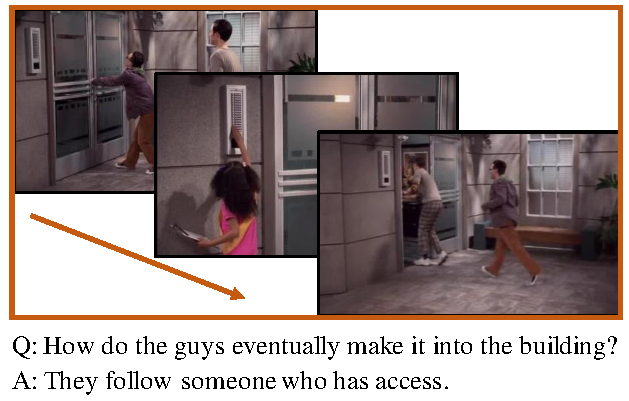
\includegraphics[height=5.8cm]{figure/c1_1.pdf}
\subcaption{视频问答举例}
\label{fig:c1_videoqa_example}
\end{subfigure}
\begin{subfigure}[b]{0.39\linewidth}
\centering
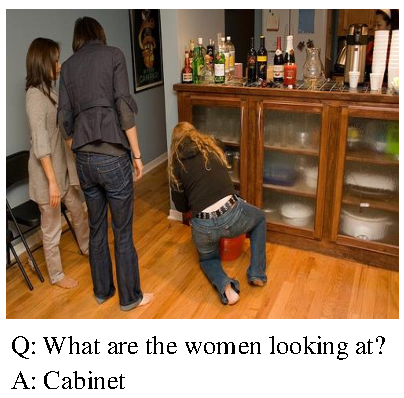
\includegraphics[height=5.8cm]{figure/c1_2.pdf}
\subcaption{视觉问答举例}
\label{fig:c1_vqa_example}
\end{subfigure}
\caption{典型视觉问答示例}
\label{fig:c1_vqa} 
\end{figure}
% ********************************************************************


% ******************************************************************
\xsection{面临的挑战}{Research Challenge}
% ******************************************************************


% 基于图像的视觉问答任务~\cite{antol2015vqa} 要求模型根据给定的图像和问题自动推理并生成问题的答案。
% 本文依据模型中使用的主要技术将
% 当前的视觉问答方法可大体分为基于图网络的视觉问答方法、基于多模态预训练模型的视觉问答方法以及传统的视觉问答方法。
当前主流的视觉问答方法是基于图网络的方法~\cite{wu2018object,cadene2019murel,li2019relation,hu2019language,huang2020location,kim2020modality,wang2021dualvgr,seo2021attend,park2021bridge}和基于多模态预训练模型的方法~\cite{lu2019vilbert,su2019vl,li2019visualbert,chen2020uniter,tan2019lxmert,li2020oscar,cho2021unifying,jin2022good,jiang2022finetuning,zeng2022multi,li2022blip,wang2022ofa}。
基于图网络的方法从任务的初衷出发,致力于对输入的视觉内容进行充分的理解,通过建模图像或视频中细粒度的视觉关系获得高阶的语义信息。
这类方法显著提升了模型的推理能力,以及回答语义复杂问题的能力。
基于多模态预训练模型的方法利用预训练过程中从大规模视觉文本数据中获得的丰富知识和各种Transformer~\cite{vaswani2017attention}结构显著地提高了下游视觉问答任务的性能,特别是在标准视觉问答数据集上的性能已经超过了人类水平。
尽管视觉问答在近年来已取得一系列突破性的进展,但目前计算机模型的表现与人类的表现还相差甚远,远远没有达到大规模普及和落地应用的水平。
这主要源于现实应用场景的复杂性,这种复杂性导致可能提出的问题更加多样化、所需的答案无法预先定义,以及能提供的标注数据非常有限。
因此,本文将从推动视觉问答系统实用性的角度出发系统地分析视觉问答所面临的一系列挑战:

\begin{itemize}[wide,leftmargin=0pt,itemsep=1pt]
\item\textbf{对视频中多粒度视觉语言信息的利用不充分。} 视频通常以多媒体的形式呈现,具有丰富的时空信息和文本字幕,这为视频问答带来了极大的问题多样性。在回答视频相关的问题时,可能需要模型理解视频片段中所描述的全局事件,或是理解视频某些帧中人物之间的细粒度交互关系,甚至需要需要对视频的字幕进行多粒度的理解。然而,目前的方法更多聚焦于对视频视觉内容的多尺度表征与理解,对于视频文本字幕的处理则往往停留在全局表征的层面,这在一定程度上忽视了对视频语言内容的多粒度表征,导致模型对视频中多粒度视觉语言信息利用不充分。因此,如何在不同尺度上同等程度地表征视频的视觉和语言内容,以便灵活应对多样化的问题,是当前视觉问答模型所面临的一项重要挑战。

\item\textbf{语言偏见导致的泛化能力不足。} 虽然视觉问答模型在标准数据集上已取得诸多进展,但要使视觉问答模型能够自适应地泛化到分布外样本仍然是一个巨大的挑战。当前大多数视觉问答方法通常处理具有相似数据分布的训练集和测试集。在这样独立同分布的设置下训练和测试视觉问答模型会使模型性能很大程度上受到数据中语言偏见的影响。目前的视觉问答去偏方法大都基于已知偏见,即考虑语言偏见的先验知识(统计信息),并在此基础上设计了针对性的去偏方法,以减少数据集中显式存在的偏见。相较之下,基于未知偏见的方法除了通过使用人工标注新数据来平衡和减少偏见外,大多采用了数据增强和对抗训练的策略。这些基于未知偏见的方法虽然在一定程度上独立于特定数据集,具有更高的实用性,但仍然存在一些不足,如人工标注数据的数据增强方式过于耗时,以及对抗训练的稳定性不足等。因此,如何在无需利用特定数据集的统计先验且不进行数据增强的情况下提升模型生成分布外答案的能力,是当前视觉问答模型亟待解决的一项重要挑战。

% 这使得视觉语言预训练带来的视觉问答鲁棒性的提升相对有限,远低于对视觉问答精度的提升。
\item\textbf{对视觉语言输入变化的鲁棒性不足。} 最近,大规模视觉语言预训练技术显著提升了下游视觉问答任务的性能,使视觉问答模型在标准数据集上的性能达到甚至超过了人的水平。然而,用有限的数据对极大规模的视觉语言预训练模型进行微调常常会导致过拟合和泛化能力不足,从而影响模型的鲁棒性。从信息论的角度分析,模型鲁棒性不足的原因可能在于视觉语言预训练模型生成的表征不可避免地包含与下游视觉问答任务无关的和冗余的信息。无关的信息会鼓励视觉问答模型学习表征和标签之间统计上的虚假关联,与任务无关的冗余信息会降低视觉问答系统对输入变化的敏感度。这两种信息都可能损害模型对视觉语言输入变化的敏感性和适应性,进一步降低视觉问答模型的输入鲁棒性。因此,在将视觉语言预训练模型迁移至视觉问答任务时,如何简单有效地提高模型的输入鲁棒性成为了当前基于多模态预训练模型视觉问答方法所面临的一项重要挑战。


\item\textbf{低资源场景下学习能力不足。} 大规模视觉语言预训练模型采用“先预训练后微调”的方式,显著提升了下游视觉问答任务的性能。标准的微调是在给定的下游任务上微调预训练模型的所有参数。随着预训练模型规模的不断扩大,这种参数调节机制极大地增加了计算和存储成本,在低资源场景下面临过拟合等问题。一种关键的解决方案是进行参数有效微调,即在保持大部分预训练模型权重冻结仅更新部分模型参数或在预训练模型中添加轻量级的可训练模块。尽管现有的有效参数微调方法大大减少了可调参数的数量,但其性能尚未达到全模型微调的水平。特别是在低资源场景下,现有的参数有效微调方法在性能上远不如全模型微调。因此,在低资源场景下,如何提高参数有效微调方法的有效性,使得基于视觉语言预训练模型的视觉问答性能达到甚至超过全模型微调,是亟待解决的一项挑战。

\end{itemize}


% ******************************************************************
\xsection{本文研究内容}{Research Content}

为了解决上述挑战,本文对基于图网络和多模态预训练模型的视觉问答方法展开了系统研究。首先,本文聚焦于如何有效利用图网络的推理和生成能力,以增强模型对多粒度信息的利用率和分布外泛化能力,进而提出了两种基于图网络的方法。然后,本文探讨如何有效地运大规模视觉语言预训练模型丰富的先验与知识,以提高模型对输入变化的敏感性和少样本学习能力,从而提出了两种基于多模态预训练模型的方法。如图~\ref{fig:c1_arrangement}所示,本文的四个研究内容分别对应了上述四个挑战,具体研究内容如下:

\begin{itemize}[wide,leftmargin=0pt,itemsep=1pt]
\item \textbf{提出了基于多粒度视觉语言推理的视频问答方法。} 针对视频问答模型对多粒度视觉语言信息利用不充分的问题,本文从视频理解的角度出发探讨一个完备的视频问答模型所应具备的基本功能,即在不同的尺度上同等程度地表征视频的视觉和语言内容并在表征整合时兼顾表征的多样性,以应对问题的多样性。因此,本文提出了基于多粒度视觉语言推理的视频问答方法。该方法设计的核心思路是利用图统一视觉和语言的多尺度编码及多样性表征的整合。具体来说,该方法首先使用基于图的视觉和语言编码器在不同的语义层面分别对视频的视觉和语言内容进行编码,生成多粒度的视觉和语言表征。然后,将获得的多粒度视觉和语言表征以及问题表征传递到多样性感知的视觉语言推理模块进行整合。在保留表征判别性的同时自适应地学习不同表征的重要性,提升了跨模态表征融合的有效性。本文在开放式和多选式视频问答数据集上进行了广泛的实验。实验结果表明在不增加模型参数量的情况下本文方法能更有效地整合多粒度视觉语言表征,提高了对多粒度视觉语言信息,特别是语言信息的利用率。


\item \textbf{提出了基于图生成建模的视觉问答分布外泛化方法。} 针对语言偏见导致视觉问答模型泛化能力不足的问题,本文将视觉问答的分布外泛化问题表述为组合泛化问题,利用域内数据来生成现有视觉概念的新组合来使视觉问答模型产生分布外的答案。考虑到图生成过程中自然蕴涵的组合泛化特性,本文提出了一种基于图生成建模的训练策略。该策略具有图关系生成建模和图表征生成建模两个核心模块,并以一定的概率分别执行这两个模块,生成新的关系矩阵或新的节点表征来促使基线视觉问答模型泛化到分布外样本。此外,为了缓解图生成建模过程中的不稳定梯度问题,本文还提出了梯度分布一致性损失来约束具有对抗性扰动的数据分布和生成的数据分布的梯度一致性。本文使用多个基线视觉问答模型在不同的数据集上进行了丰富的实验。实验结果验证了所提策略在提高基线视觉问答模型分布外泛化性能时的有效性,表明从组合泛化的角度减少语言偏见、提高泛化能力的可行性。
% 本文提出利用图生成中自然蕴含的组合泛化属性进行隐式的数据增强。该算法首先对图像中的视觉目标构建目标关系图,然后分别对目标关系图中的关系矩阵和节点表征进行生成建模来生成罕见的或分布外的样本, 从而减少视觉问答数据中存在的偏见并提高模型的泛化能力。


\item \textbf{提出了基于相关信息瓶颈理论的鲁棒视觉问答方法。} 针对视觉问答模型对视觉语言输入变化鲁棒性不足的问题,本文从信息论的角度分析模型鲁棒性差的原因进而发现提高模型鲁棒性本质上就是使预训练模型获得的表征更加紧凑和更加任务相关。
因此,在为视觉问答微调预训练视觉语言模型时,本文提出了相关信息瓶颈理论来鼓励学习到的表征收敛到最小充分统计量。具体来说,该理论通过在最小化表征和模型输入之间互信息的同时最大化表征和输出之间的互信息,来促进视觉语言表征收敛到最小充分统计量。为了准确估计多模态输入和表征之间的互信息,本文为多模态输入和表征之间的互信息估计提供了紧凑的理论上界,通过度量多模态输入和表征之间的多种信息关联有效地指导视觉问答模型学习更鲁棒的表征并促进多模态对齐。
本文使用多个基线预训练视觉语言模型在五个输入鲁棒性评测数据集上进行了大量的实验,验证了所提方法对提高视觉问答模型输入鲁棒性的有效性,表明该方法能一定程度解决当前视觉问答模型对视觉语言输入变化鲁棒性不足的问题。
% 是预训练视觉语言模型生成的表征不可避免地包含了与下游视觉问答任务无关的和冗余的信息。
% 本文提出相关信息瓶颈的训练目标,旨在平衡输入表征中信息的冗余和压缩, 减少表征中任务无关的冗余信息,进而促进视觉问答模型学习更输入鲁棒的表征。


\item \textbf{提出了基于冗余感知参数有效微调的低资源视觉问答方法。} 针对视觉问答模型在低资源场景下学习能力不足的问题,本文在迁移大规模视觉语言预训练模型丰富知识至视觉问答任务时,通过参数有效微调的方式降低可训练参数的数量,以避免过拟合问题。因此,本文提出了冗余感知参数有效微调的低资源视觉问答方法。该方法向预训练模型中添加轻量的可训练模块而保持预训练模型本身参数不变,用来获取蕴涵在视觉语言预训练模型中知识和学习与特定任务相关的信息。为了进一步降低所添加模块的参数冗余,本文在低秩子空间中重参数化了专家的权重并共享了部分权重。此外,为了减少从视觉语言预训练模型中获得的与任务无关的冗余信息并鼓励专家学习更多与任务相关的信息,本文提出了基于表征冗余的训练目标以正则的方式促进模型学习更鲁棒的表征。在三个数据集上不同低资源设置下进行的广泛的实验表明,所提方法是现有唯一在所有数据集上性能都优于全模型微调的参数有效微调方法,且在在一定程度上解决了视觉问答模型低资源场景下学习能力不足的问题。

\end{itemize}


% ********************************************************************
\begin{figure}[!t]
\centering
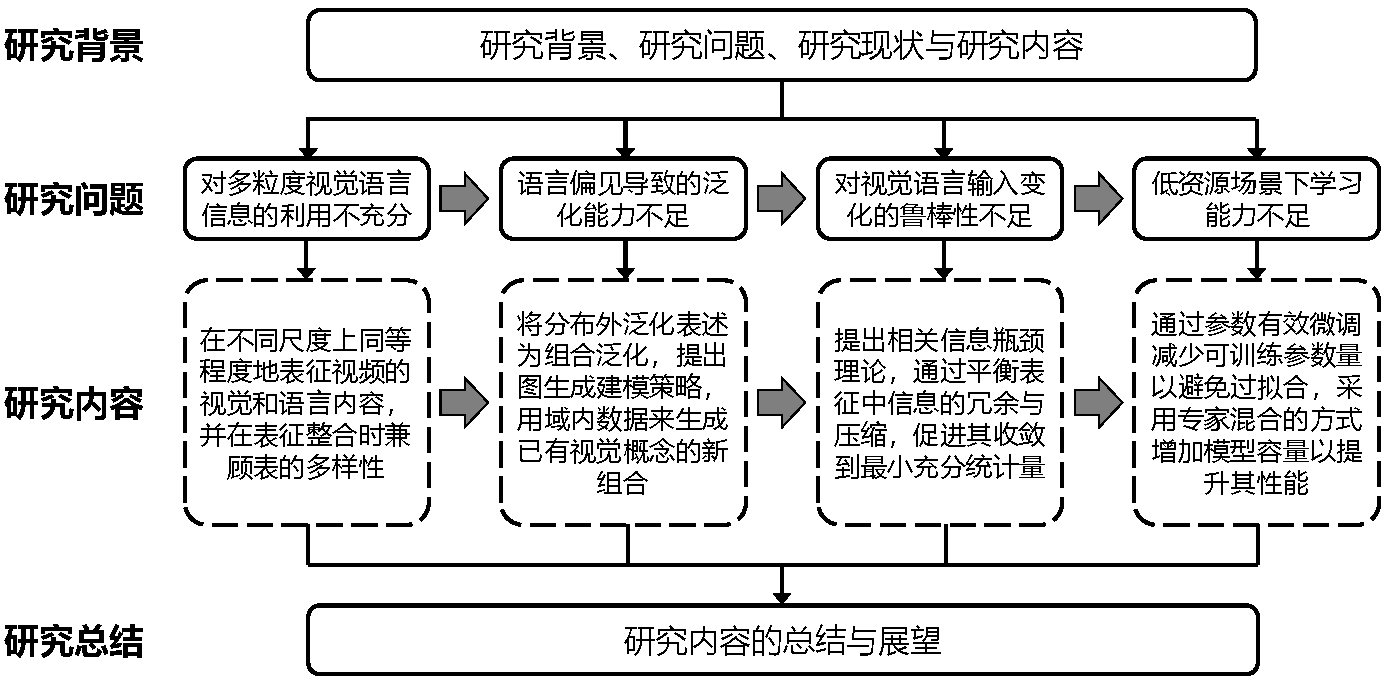
\includegraphics[width=1.0\linewidth]{figure/c1_overview.pdf}
\caption{本文的研究内容的整体框架图}
\label{fig:c1_arrangement} 
\end{figure}
% ********************************************************************

% ******************************************************************
\xsection{本文组织结构}{Arrangement}


本文进行基于图网络和多模态预训练模型的视觉问答方法的研究。
全文共七章,之后的章节安排如下: 
\begin{itemize}[wide,leftmargin=0pt,itemsep=1pt]    
\item 第二章就视频问答、视觉问答中的分布外泛化、视觉问答中的输入鲁棒性和视觉问答中的低资源学习等几方面的相关工作进行了综述。

\item 第三章介绍了基于多粒度视觉语言联合推理的视频问答方法。针对视觉问答模型对多粒度视觉语言信息利用不充分的问题,本章提出对视觉和语言输入分别进行多粒度的编码来提高对视觉语言输入中信息的发掘和表征,并提出了多样性感知的视觉语言联合推理模块对获得的多粒度多来源表征进行有效的融合。

\item 第四章介绍了基于图生成建模的视觉问答分布外泛化方法。针对语言偏见导致视觉问答模型泛化能力不足的问题,本章提出利用图生成中自然蕴含的组合泛化属性进行隐式的数据增强。该方法首先对图像中的目标构建目标关系图,然后分别对目标关系图中的关系矩阵和节点表征进行生成建模生成罕见的或分布外的样本,显著地提高了基线视觉问答模型分布外的泛化能力。

\item 第五章介绍了基于相关信息瓶颈理论的鲁棒视觉问答方法。针对视觉问答模型对视觉语言输入变化鲁棒性不足的问题,本章提出相关信息瓶颈的训练目标来平衡视觉语言预训练模型生成表征中信息的冗余和压缩,减少表征中任务无关的冗余信息,显著提高了视觉问答模型的输入鲁棒性。

\item 第六章介绍了基于冗余感知参数有效微调的低资源视觉问答方法。
针对视觉问答模型在低资源场景下学习能力不足的问题,本章提出以专家混合的方式对大规模视觉语言预训练模型进行参数有效微调,在保证低参数低存储的同时提高了模型的容量,使得在低资源视觉问答任务上,参数有效微调的性能超过了全模型微调。

\item 第七章总结全文工作并对视觉问答领域可能的研究方向进行了探讨和展望。
\end{itemize}


